\section{Current Electricity} \index{Electricity! current! Form II topic}
\label{sec:ii-current-electricity}

\begin{multicols}{2}


\section*{Simple Electric Circuits}


\subsection{Conductors and Insulators}

\begin{center}
\includegraphics[width=0.4\textwidth]{./img/conductors-insulators.png}
\end{center}

\begin{description*}
%\item[Subtopic:]{}
\item[Materials:]{Dry cells, light bulb, speaker wire, cardboard, various materials (e.g. nail, pen cap, aluminum foil, string, balloon, toothpick, bottle cap, pencil, etc.)}
\item[Setup:]{Connect the dry cells and light bulb using speaker wire and leave two ends of the wire free.}
\item[Procedure:]{Have students predict which materials will cause the bulb to light. Then try them one by one by placing them across the free wire ends.}
%\item[Hazards:]{}
%\item[Questions:]{}
\item[Observations:]{Metal objects such as nails, aluminum foil, bottle caps, etc. turn on the light, while others do not.}
\item[Theory:]{\emph{Conductors} allow electric current to pass through them easily, while \emph{insulators} do not. Placing conducting materials (e.g. many metals) across the wires closes the circuit and allows electrons to flow through the bulb and produce light.}
%\item[Applications:]{}
%\item[Notes:]{}
\end{description*}

\subsection{Student Circuits}

%\begin{center}
%\includegraphics[width=0.4\textwidth]{./img/.jpg}
%\end{center}

\begin{description*}
%\item[Subtopic:]{}
%\item[Materials:]{}
\item[Setup:]{Make a square or circular pathway using chairs/tables as boundaries on either side. Place sheets of paper with ``+'' and ``-'' written on them on one table. Place several obstacles (e.g. stools, stacks of books, etc.) throughout the path.}
\item[Procedure:]{Have students walk in one direction (from + to -) through the track. After some time, place a large obstacle (e.g. desk) at some point to block off the path.}
%\item[Hazards:]{}
%\item[Questions:]{}
%\item[Observations:]{}
\item[Theory:]{The path represents an electric circuit. The students (electrons) move around the path from the positive terminal to the negative terminal, but their motion is impeded by the obstacles (resistances). Placing the table to cut off the path represents a switch which prevents the flow of the electrons.}
%\item[Applications:]{}
%\item[Notes:]{}
\end{description*}

\columnbreak

\subsection{Creating a Light Bulb}

%\begin{center}
%\includegraphics[width=0.4\textwidth]{./img/source/.png}
%\end{center}

\begin{description*}
%\item[Subtopic:]{}
\item[Materials:]{Glass jar with lid, glue, wires, power source, thin iron wire, nail}
\item[Setup:]{Use the nail to poke two holes in the jar lid. Pass a wire through each hole half way into the jar. Connect the wires inside the jar with the iron wire. Seal the sires into the lid with glue and close the lid on the jar.}
\item[Procedure:]{Connect the wires outside the jar to the power source.}
%\item[Hazards:]{}
\item[Observations:]{If enough current is passing, the iron wire will light up, creating a light bulb for a short time until the wire burns out.}
\item[Theory:]{Electricity can be used to generate light as a result of resistance in a wire.}
\item[Questions:]{Why do bulbs eventually stop working? What other materials produce light when heated?}
%\item[Applications:]{}
\item[Notes:]{You may need to try different types of wire for the bulb. It should be very thin and have a high resistance.}
\end{description*}

%==================================================================================================%

\section*{Ohm's Law} \index{Ohm's law|see{Practicals}}


\subsection{Verifying Ohm's Law} \index{Practicals! Ohm's law}
\textbf{*NECTA PRACTICAL*}

\begin{center}
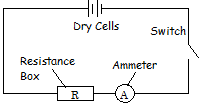
\includegraphics[width=0.4\textwidth]{./img/ohms-law.png}
\end{center}

\begin{description*}
%\item[Subtopic:]{}
\item[Materials:]{Dry cells, speaker wire, resistance box/rheostat, ammeter/galvanometer}
\item[Setup:]{Connect the circuit as shown.}
\item[Procedure:]{Adjust the resistance box/rheostat to give 1 $\Omega$. Read the current $I$ on the ammeter. Repeat for different resistances (2 $\Omega$, 3 $\Omega$, 4 $\Omega$, 5 $\Omega$).}
%\item[Hazards:]{}
\item[Questions:]{Tabulate values of $R$ and $I$. Plot a graph of resistance, $R$ (vertical) against $\frac{1}{I}$ (horizontal). Find the slope of the graph.}
\item[Observations:]{As the resistance increases, the current decreases.}
\item[Theory:]{Ohm's Law tells us that potential difference in a circuit is directly proportional to the current passing through it ($V = IR$). Solving this equation for $R$ gives $R = \frac{V}{I}$, so the slope of the graph represents the voltage $V$.}
%\item[Applications:]{}
%\item[Notes:]{}
\end{description*}

%==================================================================================================%

\section*{Electrical Components}


\subsection{Circuit Boards}

\begin{center}
\includegraphics[width=0.45\textwidth]{./img/vso/circuit-board.jpg}
\end{center}

\begin{description*}
%\item[Subtopic:]{}
\item[Materials:]{Wood board, nails}
\item[Setup:]{Make a grid of nails in the board as shown.}
\item[Procedure:]{Use the nails to connect different circuit components. Gaps between nails can serve as a switch.}
%\item[Hazards:]{}
%\item[Questions:]{}
%\item[Observations:]{}
%\item[Theory:]{}
%\item[Applications:]{}
%\item[Notes:]{}
\end{description*}

\subsection{Switches}

\begin{center}
\includegraphics[width=0.49\textwidth]{./img/vso/switches.jpg}
\end{center}

\begin{description*}
%\item[Subtopic:]{}
\item[Materials:]{Nails, small wooden blocks, paper clips, speaker wire}
%\item[Setup:]{}
\item[Procedure:]{Assemble the various switches shown and use them to connect circuit components.}
%\item[Hazards:]{}
%\item[Questions:]{}
%\item[Observations:]{}
%\item[Theory:]{}
%\item[Applications:]{}
%\item[Notes:]{}
\end{description*}

\columnbreak

\subsection{Rheostat}

\begin{center}
\includegraphics[width=0.49\textwidth]{./img/vso/rheostat.jpg}
\end{center}

\begin{description*}
%\item[Subtopic:]{}
\item[Materials:]{Dry cell, metal strip, pencil, wire, bulb}
%\item[Setup:]{}
\item[Procedure:]{Cut a pencil in half so that its graphite center is showing. Connect a dry cell, bulb and metal strip as shown. Move the metal strip along the graphite in the pencil.}
%\item[Hazards:]{}
%\item[Questions:]{}
\item[Observations:]{When the metal strip is moved to the left along the graphite of the pencil, the bulb burns more brightly.}
\item[Theory:]{The graphite acts as a resistor. Its resistance depends on its length, so when a shorter distance is used in the circuit, there is less resistance and the bulb burns more brightly.}
%\item[Applications:]{}
%\item[Notes:]{}
\end{description*}

\subsection{Finding Circuit Components}

%\begin{center}
%\includegraphics[width=0.4\textwidth]{./img/source/.png}
%\end{center}

\begin{description*}
%\item[Subtopic:]{}
\item[Materials:]{Old or broken electronics (radio, car stereo, computer, phone charger, disc drive, etc.), pliers, screw driver, soldering iron (optional), empty matchboxes}
\item[Setup:]{Ask local community members/fundis/repair shops for old or broken electronics. }
\item[Procedure:]{Identify common components inside the devices and place them in separate containers (matchboxes). Pliers or a soldering iron may be necessary to remove some components.}
\item[Hazards:]{If using a soldering iron, do not touch the tip as it can quickly cause second degree burns. NEVER open a component which is connected to a power source!}
%\item[Questions:]{}
\item[Observations:]{You should be able to find a variety of resistors, capacitors, wires, motors, rheostats, switches, diodes, transistors, transformers, speakers, inductors, bulbs, etc.}
%\item[Theory:]{}
%\item[Applications:]{}
\item[Notes:]{Have this be an ongoing activity for your school. Keep looking for more things to take apart.}
\end{description*}

\columnbreak

%==================================================================================================%

\section*{Water Analogies}


\subsection*{Switches}

\begin{center}
\includegraphics[width=0.5\textwidth]{./img/vso/analogy-switch.jpg}
\end{center}

The drawbridge acts as a switch.

\begin{center}
\includegraphics[width=0.5\textwidth]{./img/vso/analogy-switch-2.jpg}
\end{center}

The plank can only be in one of
two positions. It is analogous to a
two-way switch.


\subsection*{Circuits in Series}

\begin{center}
\includegraphics[width=0.5\textwidth]{./img/vso/analogy-series.jpg}
\end{center}

lf the bridge breaks, the flow stops, i.e. if one component breaks, the
circuit is incomplete and electricity cannot flow.

\vfill
\columnbreak

\subsection*{Circuits in Parallel}

\begin{center}
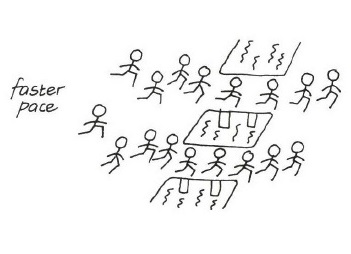
\includegraphics[width=0.5\textwidth]{./img/vso/analogy-parallel.jpg}
\end{center}

If one bridge breaks the race can go on, i.e. if one component fails
there is still an alternative route for the electricity to flow.

\subsection*{Electricity}

\begin{center}
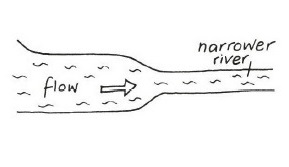
\includegraphics[width=0.5\textwidth]{./img/vso/analogy-elec.jpg}
\end{center}

The river (electricity) flows
through the narrow and the wide
part of the river. However, where
the river is narrow the amount of
water flowing (the current) is
smaller, but the resistance or
power is greater, while the
voltage stays the same.

A dam acts like a switch. Unless the dam is opened no water can flow.



\end{multicols}

\pagebreak